\documentclass[aspectratio=43]{beamer}
\usepackage[utf8]{inputenc}
\usepackage[T1]{fontenc}
\usepackage[ngerman]{babel}
\usetheme{default}
\usepackage{float}
\usepackage{graphicx}
\usepackage{ulem}
\usepackage{pgf}
\usepackage{tikz}
\usetikzlibrary{arrows,automata}
\usepackage{listings}
\lstset{frame=single,basicstyle=\scriptsize}
\usepackage{latexsym,amssymb,eurosym,amsmath,amstext}
\usepackage{multirow}
\usepackage{longtable}
\usepackage{fancyvrb}
\usepackage{pgfpages}
\usepackage{hyperref}
\setlength{\fboxsep}{0pt}
\setlength{\fboxrule}{.5pt}

\makeatletter
\renewcommand{\insertslideintonotes}[1]{{%
  \begin{pgfpicture}{0cm}{0cm}{#1\paperwidth}{#1\paperheight}
    \begin{pgflowlevelscope}{\pgftransformscale{#1}}%
      {\pgftransformshift{\pgfpointorigin}\pgftext[left,bottom]{}}
      \color{normal text.fg}
      {\pgftransformshift{\pgfpoint{\beamer@origlmargin}{\footheight}}\pgftext[left,bottom]{\copy\beamer@frameboxcopy}}
    \end{pgflowlevelscope}
  \end{pgfpicture}%
  }}
\makeatother

\AtBeginSection[]{
	\frame{\frametitle{Gliederung}\tableofcontents[currentsection,subsections]}
}

\setbeamertemplate{footline}[frame number]
\setbeamertemplate{bibliography item}[text]
%\setbeamertemplate{note page}[plain]
\setbeamercovered{transparent}
%\setbeameroption{show notes on second screen=right}

\title{LocalTwitter\\(Abschlusspräsentation)}
\author{Gruppe bluemoep\\Internet-Technologien SS2014}
\date{29. Juli 2014}
 
\begin{document}
\frame{\maketitle}
\frame{\tableofcontents[subsections,hideothersubsections]}

\section{Entwurf}
\begin{frame}
	\frametitle{Desktop}
	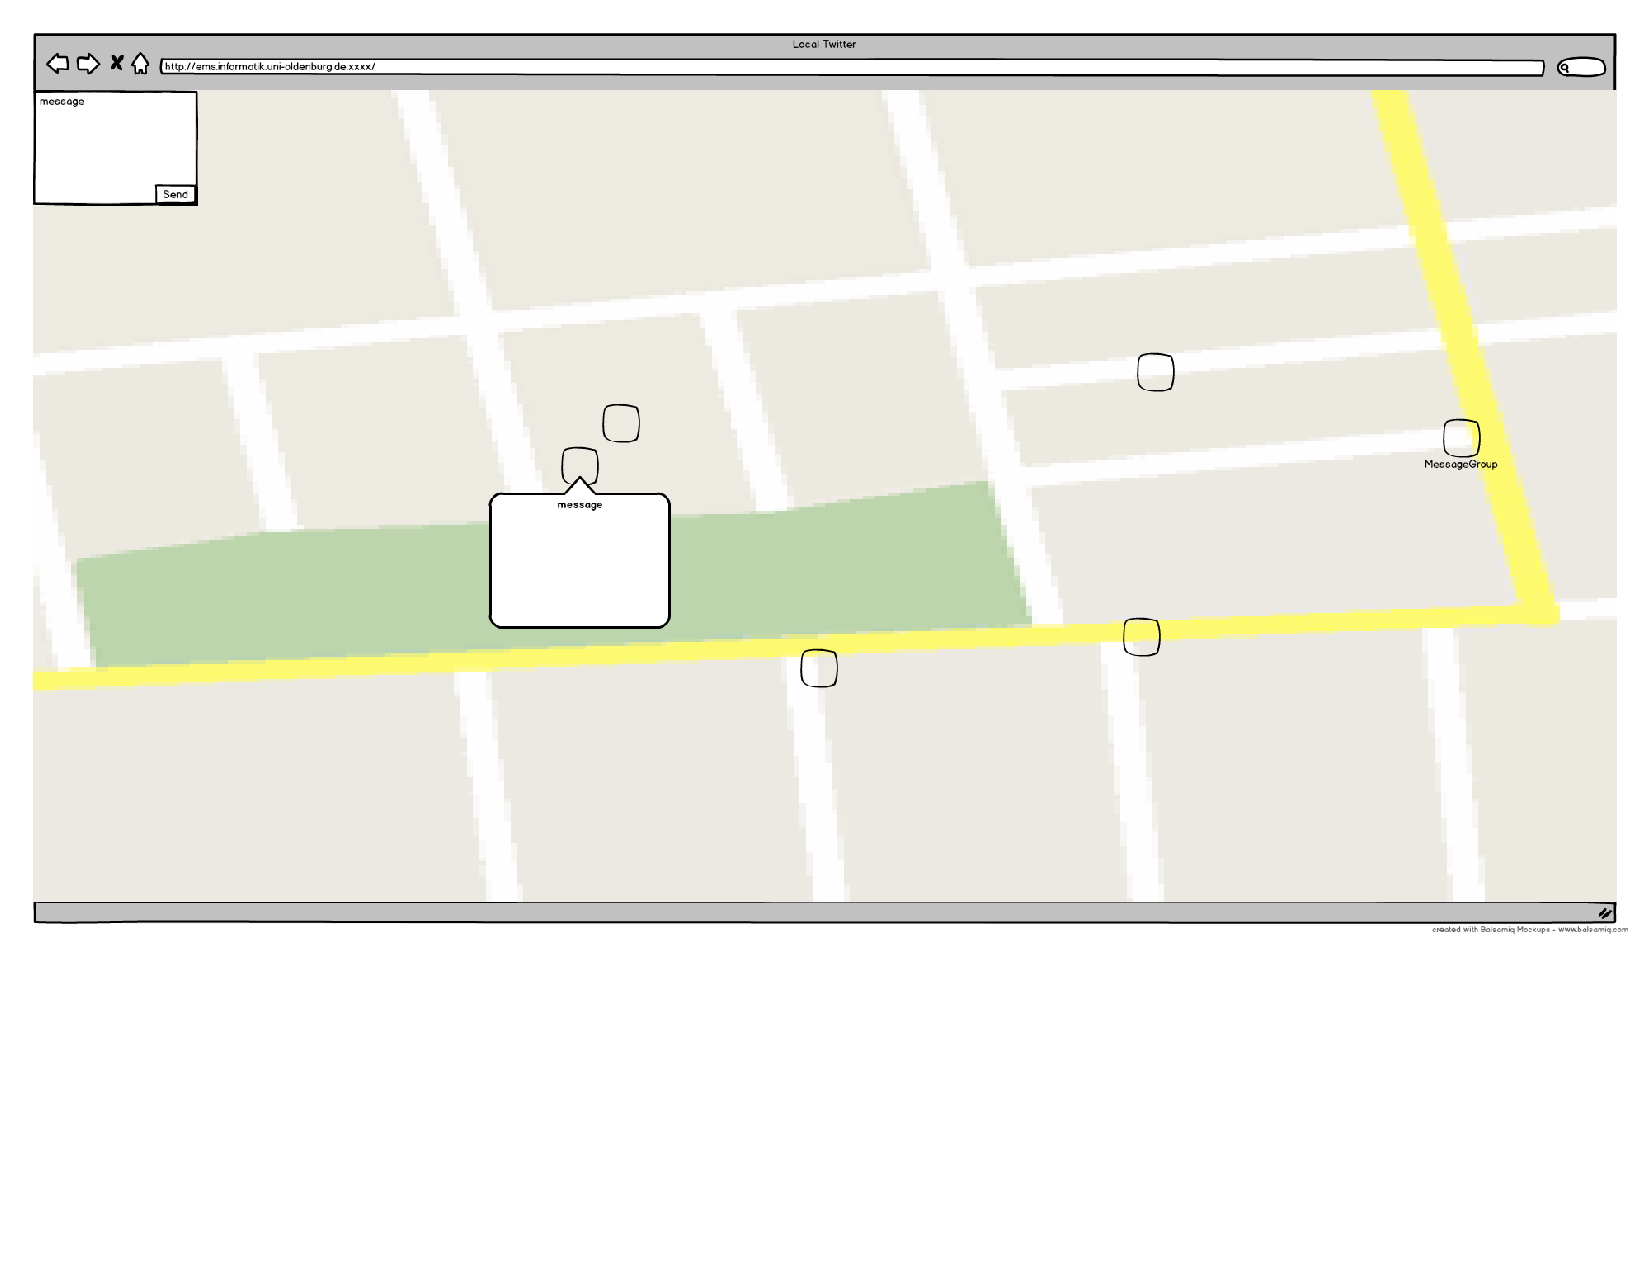
\includegraphics[width=\textwidth]{ITDesktopMockUp.pdf}
\end{frame}

\begin{frame}
	\frametitle{Mobile}
	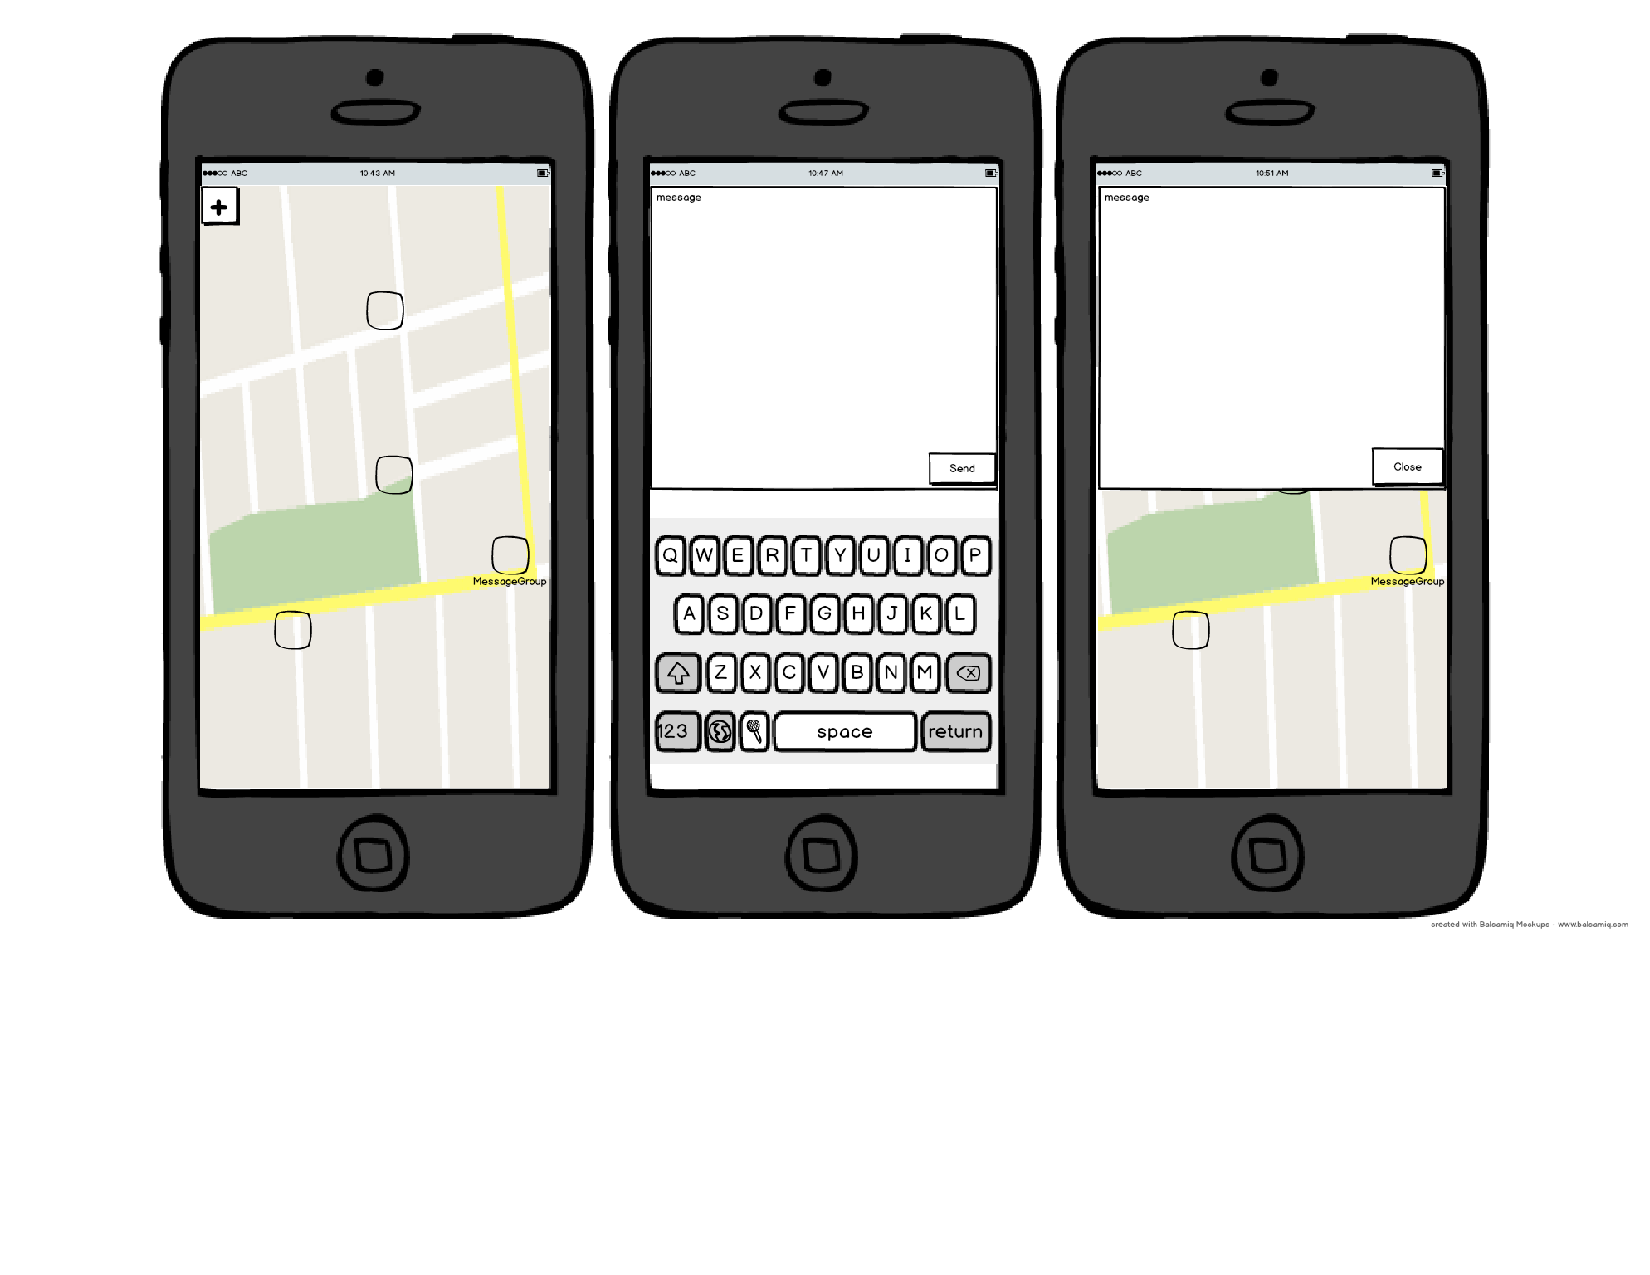
\includegraphics[width=\textwidth]{ITMobileMockUp.pdf}
\end{frame}

\section{Client}
\begin{frame}
	\frametitle{Desktop (Erste Umsetzung)}
	\fbox{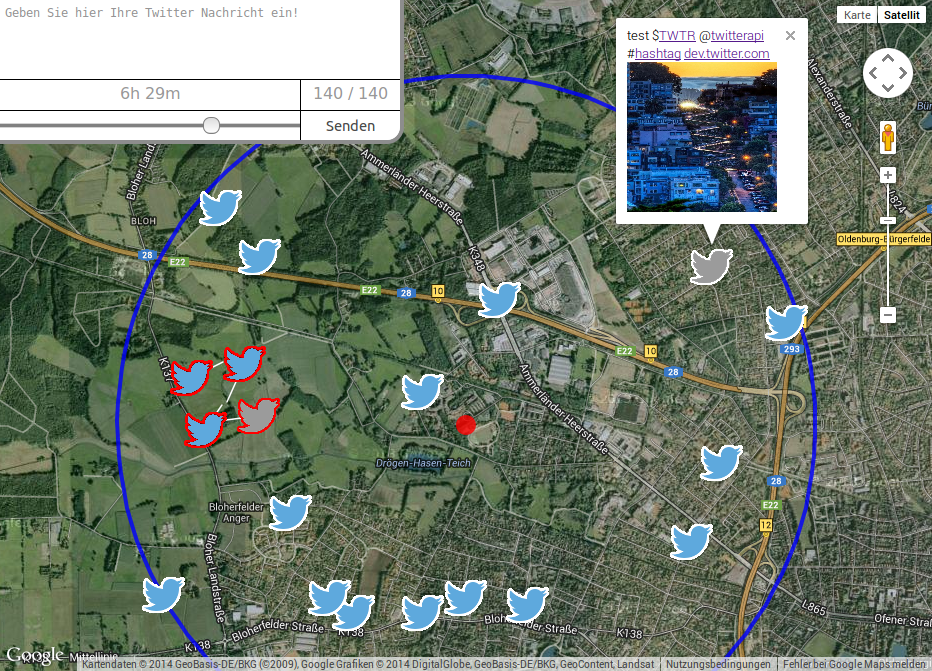
\includegraphics[width=\textwidth]{Desktop.png}}
\end{frame}

\begin{frame}
	\frametitle{Desktop (Finale Umsetzung)}
	\fbox{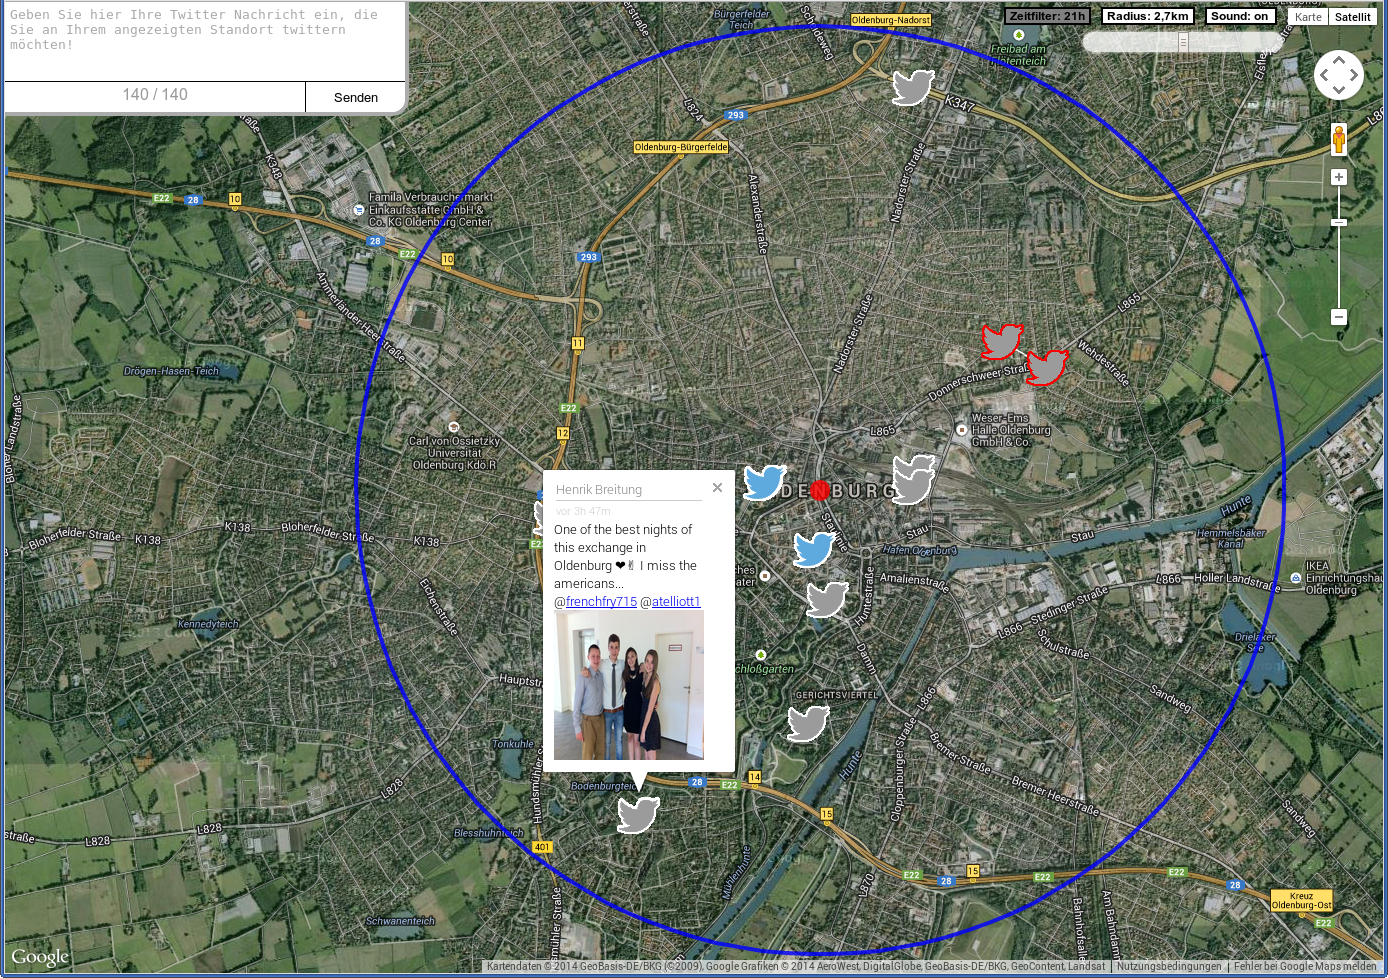
\includegraphics[width=\textwidth]{DesktopFinal.png}}
\end{frame}

\begin{frame}
	\frametitle{Mobile}
	\begin{columns}
		\column[t]{.5\textwidth}
			\fbox{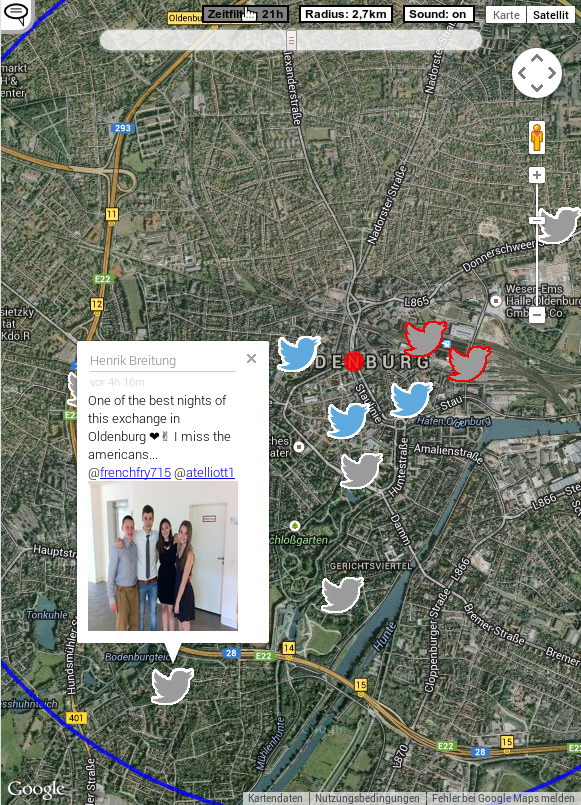
\includegraphics[width=\textwidth]{Mobile2.png}}
		\column[t]{.5\textwidth}
			\fbox{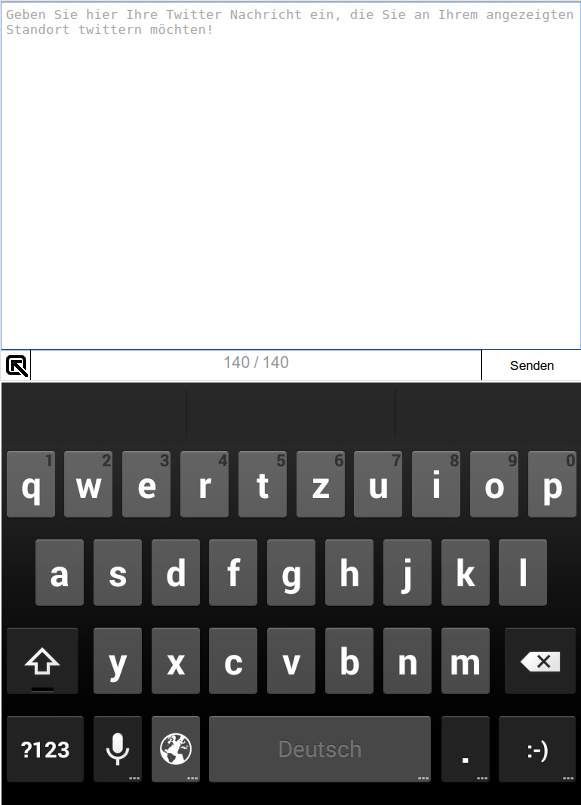
\includegraphics[width=\textwidth]{MobileInput2.png}}
	\end{columns} 
\end{frame}

\begin{frame}
	\frametitle{Features}
	\begin{columns}
		\column[t]{.5\textwidth}
			\begin{itemize}
			\item Overlays
			\item GeoLocation
			\item Zeit-Filter (logarithmisch)
			\item Radius-Filter
			\item Zeichenlimit
			\item MessageReadStorage
				\begin{itemize}
				\item LocalStorage
				\item Räumt sich auf
				\end{itemize}
			\item TweetParser
			\item Eigene Icons
			\item Overlapping-Markers-Spiderfier
			\end{itemize}
		\column[t]{.5\textwidth}
			\begin{itemize}
			\item Anzeige der eigenen Position inkl. 2km Radius
				\begin{itemize}
					\item Nachrichten nur innerhalb des Radius
				\end{itemize}
			\item Toasts
			\end{itemize}
			\rule{\textwidth}{\fboxrule}
			\begin{itemize}
			\item Objekt-Orientierter Ansatz in JavaScript
			\item Viele Klassen als Singleton
			\end{itemize}
	\end{columns}
\end{frame}

\section{Kommunikationswege}
\begin{frame}
	\frametitle{Kommunikationswege}
	\begin{tikzpicture}[->,>=stealth',shorten >=1pt,auto,node distance=4.5cm,thick,main node/.style={circle,fill=blue!20,draw,font=\sffamily\bfseries}]
	\node[main node] (1) {Client};
	\node[main node] (2) [right of=1] {Server};
	\node[main node] (3) [right of=2] {Twitter};
	
	\path[every node/.style={font=\sffamily\tiny}]
		(1)	edge [bend right] node[below] {Neue Nachricht} (2)
			edge [bend left] node[above] {Websocket: Location \& Filter Update} (2)
		(2)	edge node {Websocket: Nachrichten} (1)
			edge [bend right] node[below] {Neue Nachricht} (3)
			edge [<->, bend left] node[above] {Nachrichtenhistorie} (3)
		(3)	edge node {Streaming-API} (2);
	\end{tikzpicture}
\end{frame}

\begin{frame}
	\frametitle{„FullRequest“}
	\begin{tikzpicture}[->,>=stealth',shorten >=1pt,auto,node distance=4.5cm,thick,main node/.style={circle,fill=blue!20,draw,font=\sffamily\bfseries}]
	\node[main node] (1) {Client};
	\node[main node] (2) [right of=1] {Server};
	\node[main node] (3) [right of=2] {Twitter};
	
	\path[every node/.style={font=\sffamily\tiny}]
		(1)	edge [bend right] node[below] {Neue Nachricht} (2)
			edge [red,bend left] node[above] {Websocket: Location \& Filter Update} (2)
		(2)	edge [red] node {Websocket: Nachrichten} (1)
			edge [bend right] node[below] {Neue Nachricht} (3)
			edge [red,<->, bend left] node[above] {Nachrichtenhistorie} (3)
		(3)	edge node {Streaming-API} (2);
	\end{tikzpicture}
\end{frame}

\begin{frame}
	\frametitle{Nachricht senden}
	\begin{tikzpicture}[->,>=stealth',shorten >=1pt,auto,node distance=4.5cm,thick,main node/.style={circle,fill=blue!20,draw,font=\sffamily\bfseries}]
	\node[main node] (1) {Client};
	\node[main node] (2) [right of=1] {Server};
	\node[main node] (3) [right of=2] {Twitter};
	
	\path[every node/.style={font=\sffamily\tiny}]
		(1)	edge [red,bend right] node[below] {Neue Nachricht} (2)
			edge [bend left] node[above] {Websocket: Location \& Filter Update} (2)
		(2)	edge node {Websocket: Nachrichten} (1)
			edge [red,bend right] node[below] {Neue Nachricht} (3)
			edge [<->, bend left] node[above] {Nachrichtenhistorie} (3)
		(3)	edge node {Streaming-API} (2);
	\end{tikzpicture}
\end{frame}

\begin{frame}
	\frametitle{Nachrichten empfangen}
	\begin{tikzpicture}[->,>=stealth',shorten >=1pt,auto,node distance=4.5cm,thick,main node/.style={circle,fill=blue!20,draw,font=\sffamily\bfseries}]
	\node[main node] (1) {Client};
	\node[main node] (2) [right of=1] {Server};
	\node[main node] (3) [right of=2] {Twitter};
	
	\path[every node/.style={font=\sffamily\tiny}]
		(1)	edge [bend right] node[below] {Neue Nachricht} (2)
			edge [bend left] node[above] {Websocket: Location \& Filter Update} (2)
		(2)	edge [red] node {Websocket: Nachrichten} (1)
			edge [bend right] node[below] {Neue Nachricht} (3)
			edge [<->, bend left] node[above] {Nachrichtenhistorie} (3)
		(3)	edge [red] node {Streaming-API} (2);
	\end{tikzpicture}
\end{frame}

\section{Live-Demo}


\section{Anforderungen}
\begin{frame}[allowframebreaks]
	\frametitle{Anforderungen}
	\begin{longtable}{rl}
		\endfirsthead
		Anforderung & Erfüllt? \endhead
		\endlastfoot
		\endfoot
		Projektaufgabe vollständig gelöst & 
\includegraphics[width=12pt]{ok.png} \\
		Usability Guidelines & 
\includegraphics[width=12pt]{ok.png} \\
		Ästhetisches \& gebrauchstaugliches Design & 
\includegraphics[width=12pt]{ok.png} \\
		Relevanter Eigenanteil an Programmierung & 
\includegraphics[width=12pt]{ok.png} \\
		Keine Bibliotheken & 
\includegraphics[width=12pt]{maybe.png} \\
		Unterstützung aktueller Webbrowser & 
\includegraphics[width=12pt]{ok.png}
	\end{longtable}
	\begin{longtable}{rl}
		\endfirsthead
		Anforderung & Erfüllt? \endhead
		\endlastfoot
		\endfoot
		HTML, CSS, JavaScript, HTML-Formular, Client-Storage & 
\includegraphics[width=12pt]{ok.png} \\
		HTML5 Medienelement & 
\includegraphics[width=12pt]{ok.png} \\
		Verwendung asynchroner Kommunikation & 
\includegraphics[width=12pt]{ok.png} \\
		Anbindung eines Social-Media-Dienstes & 
\includegraphics[width=12pt]{ok.png} \\
		Zwei HTTP-Verben & 
\includegraphics[width=12pt]{ok.png} \\
		Sinnvolle Datenhaltung auf Serverseite & 
\includegraphics[width=12pt]{ok.png} \\
		Responsive Design & 
\includegraphics[width=12pt]{ok.png}
		\end{longtable}
\end{frame}


%\begin{frame}[allowframebreaks]
%	\frametitle{Literaturverzeichnis}
%	\tiny
%	\printbibliography
%\end{frame}

\end{document}
